\documentclass[10pt,a4paper]{article}

\usepackage[T1]{fontenc}
\usepackage[utf8]{inputenc}
\usepackage{lmodern}
\usepackage[margin=0.68in,top=0.62in,bottom=0.65in,includeheadfoot]{geometry}
\usepackage{microtype}
\usepackage{amsmath,amssymb}
\usepackage{booktabs,tabularx,array,graphicx}
\usepackage{float}
\usepackage[font=small,labelfont=bf]{caption}
\usepackage{xcolor}
\usepackage{enumitem}
\usepackage{fancyhdr}
\usepackage{titlesec}
\usepackage[hidelinks]{hyperref}

\definecolor{teal}{HTML}{0B7285}
\definecolor{orange}{HTML}{D9480F}
\definecolor{ink}{HTML}{24313A}
\definecolor{lightteal}{HTML}{E6F4F1}
\definecolor{lightgray}{HTML}{F3F5F6}

\hypersetup{
  colorlinks=true,
  linkcolor=teal,
  citecolor=teal,
  urlcolor=teal,
  pdftitle={Dynamic comparison of Monod and substrate inhibition models},
  pdfauthor={Mridul Sharma, Sneha Shandilya, Diggaj Maheshwari}
}

\setlength{\parindent}{0pt}
\setlength{\parskip}{3.2pt}
\setlist[itemize]{leftmargin=1.25em,itemsep=1pt,topsep=2pt}
\setlist[enumerate]{leftmargin=1.45em,itemsep=1pt,topsep=2pt}
\renewcommand{\arraystretch}{1.08}
\setlength{\tabcolsep}{4.5pt}

\titleformat{\section}
  {\large\bfseries\color{teal}}
  {\thesection.}{0.45em}{}
\titleformat{\subsection}
  {\normalsize\bfseries\color{ink}}
  {\thesubsection}{0.4em}{}
\titlespacing*{\section}{0pt}{8pt}{3pt}
\titlespacing*{\subsection}{0pt}{5pt}{2pt}

\pagestyle{fancy}
\fancyhf{}
\fancyhead[L]{\small\textcolor{teal}{CL 420 \textbar\ Project mid term}}
\fancyhead[R]{\small\textcolor{ink}{Mathematical modelling and simulation}}
\fancyfoot[C]{\small\textcolor{ink}{\thepage}}
\renewcommand{\headrulewidth}{0.35pt}
\renewcommand{\footrulewidth}{0pt}

\newcommand{\Ppastoris}{\textit{Pichia pastoris}}
\newcommand{\Rlipase}{\textit{Rhizopus oryzae} lipase}
\newcommand{\dd}{\,\mathrm{d}}
\newcommand{\methanol}{\text{methanol}}

\begin{document}

\begin{center}
  {\color{teal}\rule{\textwidth}{1.2pt}}\\[5pt]
  \begin{minipage}{0.98\textwidth}
    \centering
    {\fontsize{15.5}{20}\selectfont\bfseries\color{ink}
    Dynamic comparison of Monod and substrate\\[5pt]
    inhibition models for recombinant lipase\\[5pt]
    production in a methanol fed batch bioreactor\par}
  \end{minipage}\\[7pt]
  {\large\textcolor{teal}{CL 420, Introduction to Biochemical Engineering}}\\[5pt]
  \begin{tabular}{c}
    Mridul Sharma (23B0353) \quad Sneha Shandilya (23B0345) \quad Diggaj Maheshwari (23B0358)\\
    \textit{Mid term project report, 22 September 2026}
  \end{tabular}\\[5pt]
  {\color{teal}\rule{\textwidth}{0.45pt}}
\end{center}

\section{Motivation and objective}

Upstream bioprocess design requires a connection between microbial kinetics and reactor operation. The CL 420 project instructions identify growth and product kinetics, material balances, oxygen demand, and bioreactor analysis as core engineering requirements \cite{IITBProject,IITBKickoff}. These requirements are addressed through a dynamic study of recombinant \Rlipase{} production by \Ppastoris{} during methanol induction.

The objective is to determine how the choice of substrate kinetics affects predicted biomass, residual methanol, product activity, productivity, and oxygen demand under identical fed batch operating conditions. The study evaluates a Monod formulation against a substrate inhibition formulation.

The kinetic parameters, initial conditions, and operating strategies were obtained from the published work of Ponte et al. \cite{Ponte2018,PonteThesis}. The Monod formulation uses the same maximum rates and saturation constants as the reported model, while omitting the inhibition term. This provides a direct comparison between the two kinetic assumptions.

\section{Reference process and kinetic model}

The modelled process uses a methanol-utilizing \Ppastoris{} strain expressing \Rlipase{} under the methanol-induced $P_{AOX1}$ promoter. The initial conditions are $X_0=27\ \mathrm{g\,L^{-1}}$, $P_0=50\ \mathrm{U\,mL^{-1}}$, $V_0=2\ \mathrm{L}$, and $S_0=1\ \mathrm{g\,L^{-1}}$ for predefined feed profiles. The operating strategies are constant feed, constant growth, linearly increasing growth, and constant substrate concentration \cite{PonteThesis}.

The reported non-monotonic substrate relationship for growth and product formation is
\begin{equation}
  q_i(S)=q_{\max,i}\frac{S}{K_{S,i}+S+S^2/K_{I,i}},
  \label{eq:haldane}
\end{equation}
where $i$ represents either biomass growth or product formation. The corresponding Monod relationship used for comparison is
\begin{equation}
  q_i(S)=q_{\max,i}\frac{S}{K_{S,i}+S}.
  \label{eq:monod}
\end{equation}
The substrate inhibition relationship gives a maximum growth rate near $1.9\ \mathrm{g\,L^{-1}}$ and a maximum product formation rate near $3.5\ \mathrm{g\,L^{-1}}$. The Monod relationship increases towards saturation and does not represent this high-substrate decline.

\begin{table}[H]
  \centering
  \caption{Parameters used in both model formulations. Values were adopted from Ponte et al. \cite{Ponte2018,PonteThesis}.}
  \label{tab:parameters}
  \small
  \begin{tabularx}{\textwidth}{@{}l>{\raggedleft\arraybackslash}p{1.35cm}l@{\hspace{0.8em}}l>{\raggedleft\arraybackslash}p{1.35cm}l@{}}
    \toprule
    Parameter & Value & Unit & Parameter & Value & Unit \\
    \midrule
    $\mu_{\max}$ & 0.069 & $\mathrm{h^{-1}}$ & $q_{\max,P}$ & 2200 & $\mathrm{U\,g^{-1}\,h^{-1}}$ \\
    $K_{S,X}$ & 0.50 & $\mathrm{g\,L^{-1}}$ & $K_{S,P}$ & 10.0 & $\mathrm{g\,L^{-1}}$ \\
    $K_{I,X}$ & 7.5 & $\mathrm{g\,L^{-1}}$ & $K_{I,P}$ & 1.2 & $\mathrm{g\,L^{-1}}$ \\
    $Y_{S/X}$ & 5.14 & $\mathrm{g\,g^{-1}}$ & $m_{S/X}$ & 0.013 & $\mathrm{g\,g^{-1}\,h^{-1}}$ \\
    $Y_{O_2/X}$ & 0.206 & $\mathrm{mol\,g^{-1}}$ & $m_{O_2/X}$ & $6.1\times10^{-4}$ & $\mathrm{mol\,g^{-1}\,h^{-1}}$ \\
    \bottomrule
  \end{tabularx}
\end{table}

The uptake relations are
\begin{equation}
  q_S=Y_{S/X}\mu+m_{S/X}, \qquad
  q_{O_2}=Y_{O_2/X}\mu+m_{O_2/X}.
  \label{eq:uptake}
\end{equation}

\begin{figure}[t]
  \centering
  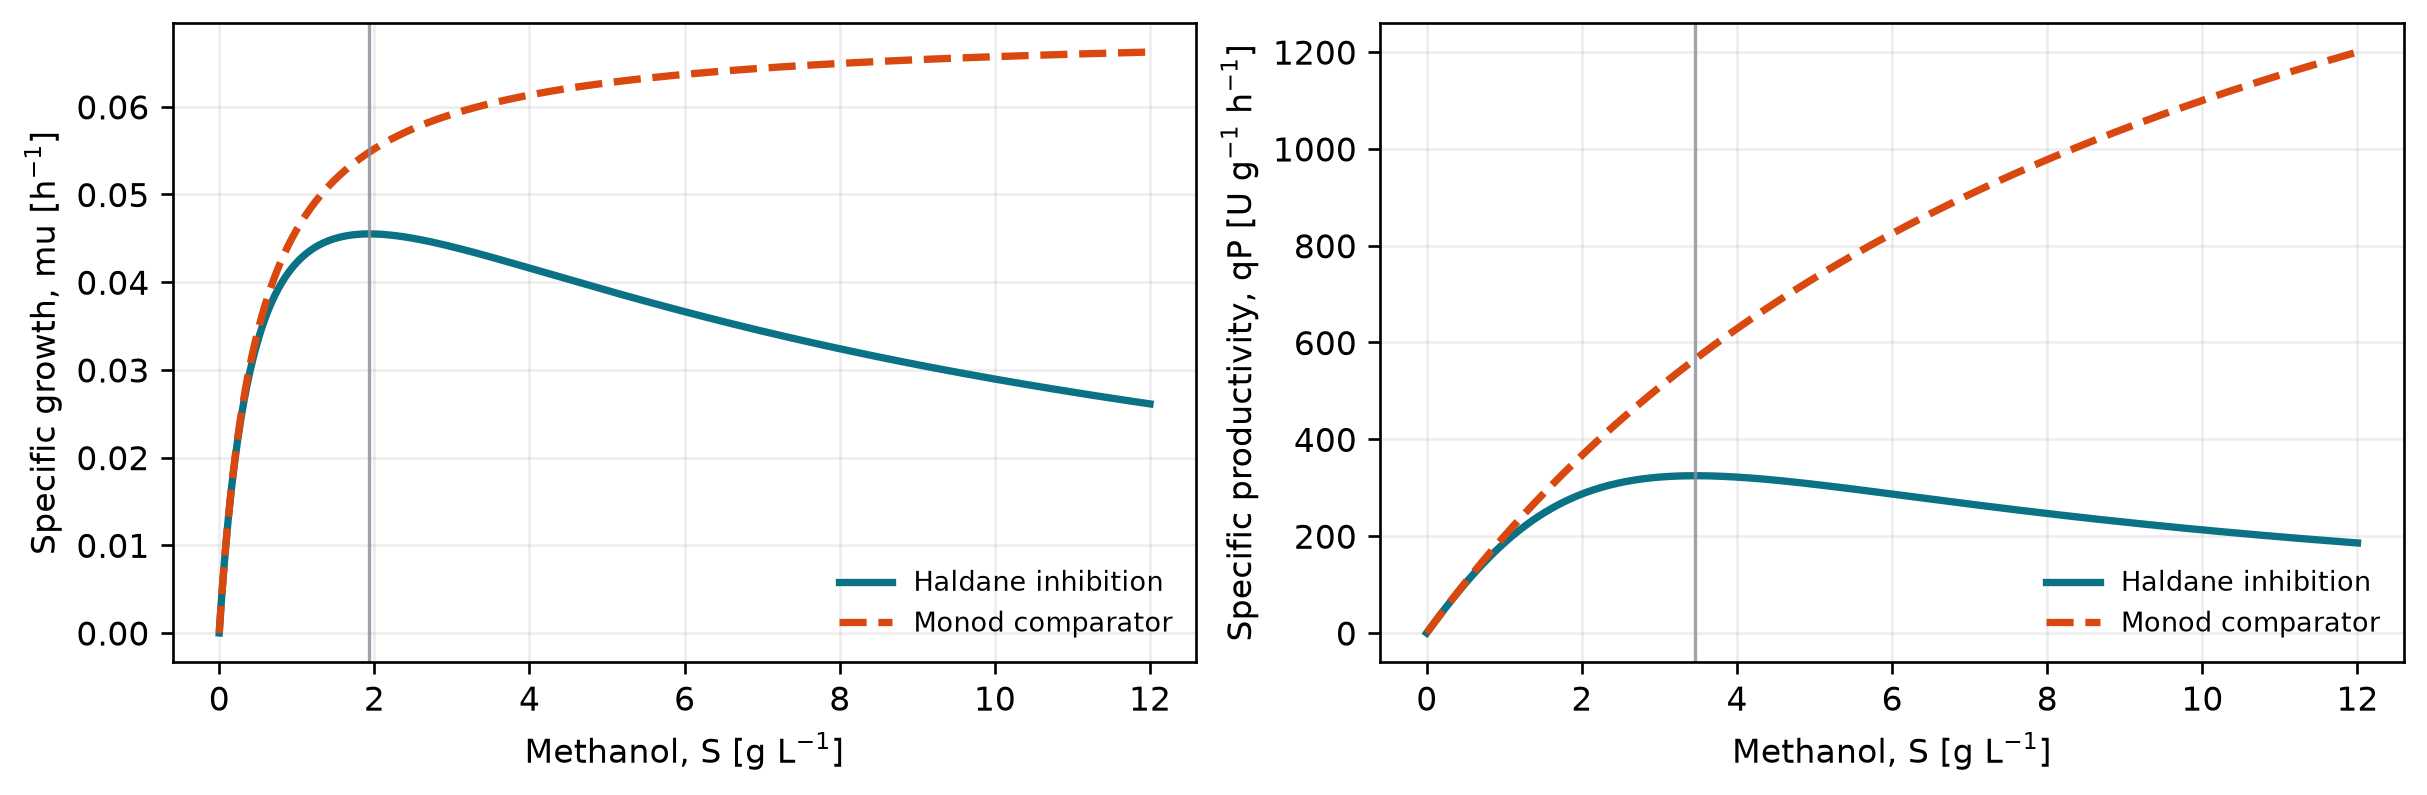
\includegraphics[width=0.83\textwidth]{figures/kinetic_laws.png}
  \caption{Specific growth and product formation laws used in the simulation. The vertical markers show the reported critical substrate concentrations for the inhibition branch.}
  \label{fig:kinetics}
\end{figure}

\section{Four state simulation method}

The dynamic state vector is $[V, XV, SV, PV]$, where $XV$ is biomass amount, $SV$ is methanol amount, and $PV$ is total product activity. With a pure methanol feed approximation, the balances are
\begin{equation}
\begin{aligned}
  \frac{\dd V}{\dd t}   &= \frac{F}{\rho_{\methanol}},\\
  \frac{\dd (XV)}{\dd t} &= \mu XV,\\
  \frac{\dd (SV)}{\dd t} &= F-q_S XV,\\
  \frac{\dd (PV)}{\dd t} &= q_P XV.
\end{aligned}
\label{eq:balances}
\end{equation}
The simulation uses $\rho_{\methanol}=792\ \mathrm{g\,L^{-1}}$. Concentrations are recovered by dividing each amount by $V$. This amount formulation makes the feed and consumption terms explicit and avoids numerical ambiguity when the working volume changes.

Four methanol feeding strategies reported by Ponte et al. \cite{Ponte2018,PonteThesis} are considered. CF uses $F=14\ \mathrm{g\,h^{-1}}$, CM targets $\mu=0.03\ \mathrm{h^{-1}}$, LM increases the target growth rate from $0.01$ to $0.04\ \mathrm{h^{-1}}$, and CS holds $S=2\ \mathrm{g\,L^{-1}}$. The CS case is implemented using the algebraic feed balance. The published sources describe an adaptive predictive PI controller but do not specify all tuned controller gains, so the ideal setpoint balance is used for this four-state analysis.

The ODEs are integrated with classical fourth order Runge Kutta at $\Delta t=0.01\ \mathrm{h}$. The process stops at the first of $X=55\ \mathrm{g\,L^{-1}}$, $V=5\ \mathrm{L}$, $S=10\ \mathrm{g\,L^{-1}}$, or $t=120\ \mathrm{h}$, matching the operating limits used in the source study. The CS result was repeated with $\Delta t=0.005\ \mathrm{h}$ as a numerical convergence check.

Oxygen demand is derived after solving the four states. The total oxygen uptake rate is
\begin{equation}
  \mathrm{OUR}=q_{O_2}XV,
  \qquad
  \mathrm{OUR}_V=q_{O_2}X,
  \label{eq:our}
\end{equation}
where OUR is in $\mathrm{mol\,h^{-1}}$ and $\mathrm{OUR}_V$ is in $\mathrm{mol\,L^{-1}\,h^{-1}}$. These quantities represent cellular oxygen demand. Oxygen transfer capacity is not evaluated in the present analysis.

\begin{figure}[t]
  \centering
  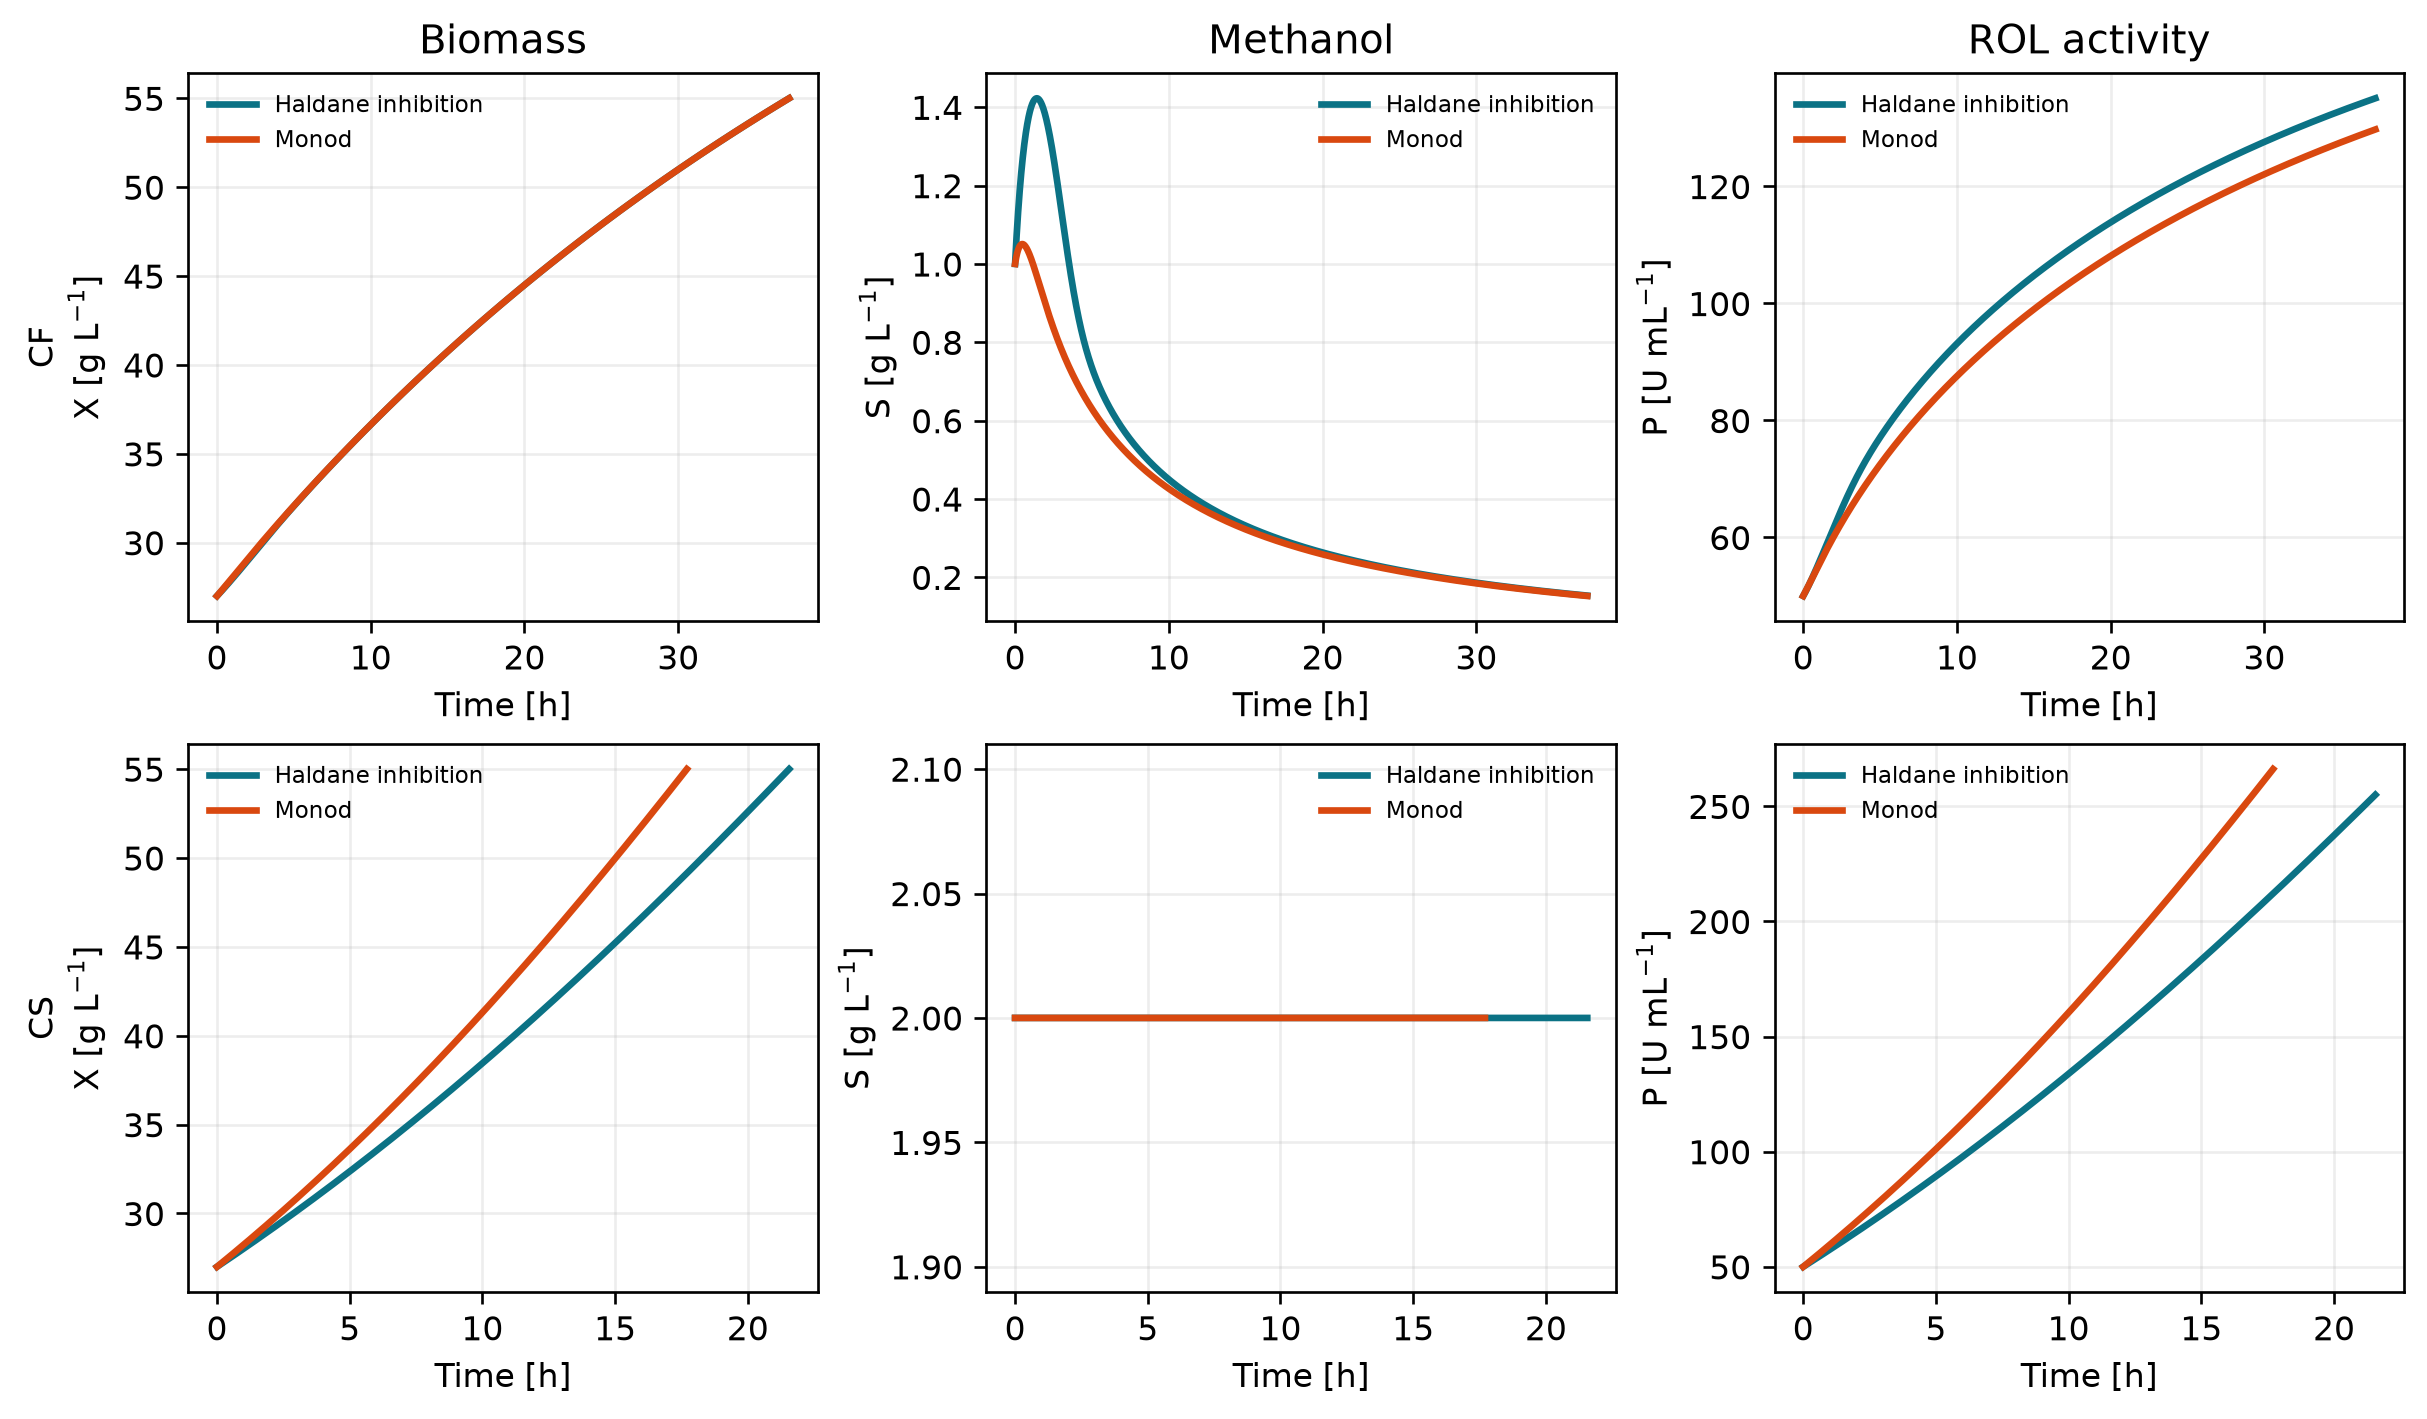
\includegraphics[width=0.98\textwidth]{figures/model_comparison.png}
  \caption{Four state comparison for constant feed CF and constant substrate CS. The same initial conditions and feed definitions are used in both branches.}
  \label{fig:comparison}
\end{figure}

\section{Simulation results}

Table~\ref{tab:results} reports the simulated values at the first process limit. The substrate inhibition and Monod formulations use the same initial conditions, feed definitions, and process limits. The results are numerical predictions generated by the present implementation.

\begin{table}[t]
  \centering
  \caption{Computed performance for the four standard strategies. $Q_P$ is the increase in total activity divided by final volume and process time. OUR$_{\max}$ is total oxygen demand.}
  \label{tab:results}
  \scriptsize
  \begin{tabular}{@{}llrrrrr@{}}
    \toprule
    Model & Strategy & $t_f$ & $P_f$ & $Q_P$ & OUR$_{\max}$ & Stop condition \\
    & & $\mathrm{h}$ & $\mathrm{U\,mL^{-1}}$ & $\mathrm{U\,L^{-1}\,h^{-1}}$ & $\mathrm{mol\,h^{-1}}$ & \\
    \midrule
    Inhibition & CF & 37.22 & 135.08 & 2619 & 0.589 & $X_{\max}$ \\
    Inhibition & CM & 32.86 & 134.64 & 2945 & 0.986 & $X_{\max}$ \\
    Inhibition & LM & 58.12 & 114.35 & 1328 & 0.838 & $X_{\max}$ \\
    Inhibition & CS & 21.56 & 255.01 & 10057 & 1.437 & $X_{\max}$ \\
    \addlinespace[1pt]
    Monod & CF & 37.22 & 129.75 & 2475 & 0.576 & $X_{\max}$ \\
    Monod & CM & 32.85 & 131.98 & 2865 & 0.986 & $X_{\max}$ \\
    Monod & LM & 58.12 & 113.73 & 1318 & 0.838 & $X_{\max}$ \\
    Monod & CS & 17.70 & 266.18 & 12870 & 1.719 & $X_{\max}$ \\
    \bottomrule
  \end{tabular}
\end{table}

Figure~\ref{fig:kinetics} shows the difference between the two kinetic formulations. Monod kinetics increases with methanol and approaches saturation, whereas the substrate inhibition formulation reaches a maximum and then declines. The growth and product peaks occur at different substrate concentrations, so a feed that supports growth is not automatically optimal for product formation.

The CS strategy gives the highest performance in both formulations. At $S=2\ \mathrm{g\,L^{-1}}$, the substrate inhibition model predicts $255.01\ \mathrm{U\,mL^{-1}}$, while the Monod formulation predicts $266.18\ \mathrm{U\,mL^{-1}}$ because it excludes substrate inhibition.

\begin{figure}[t]
  \centering
  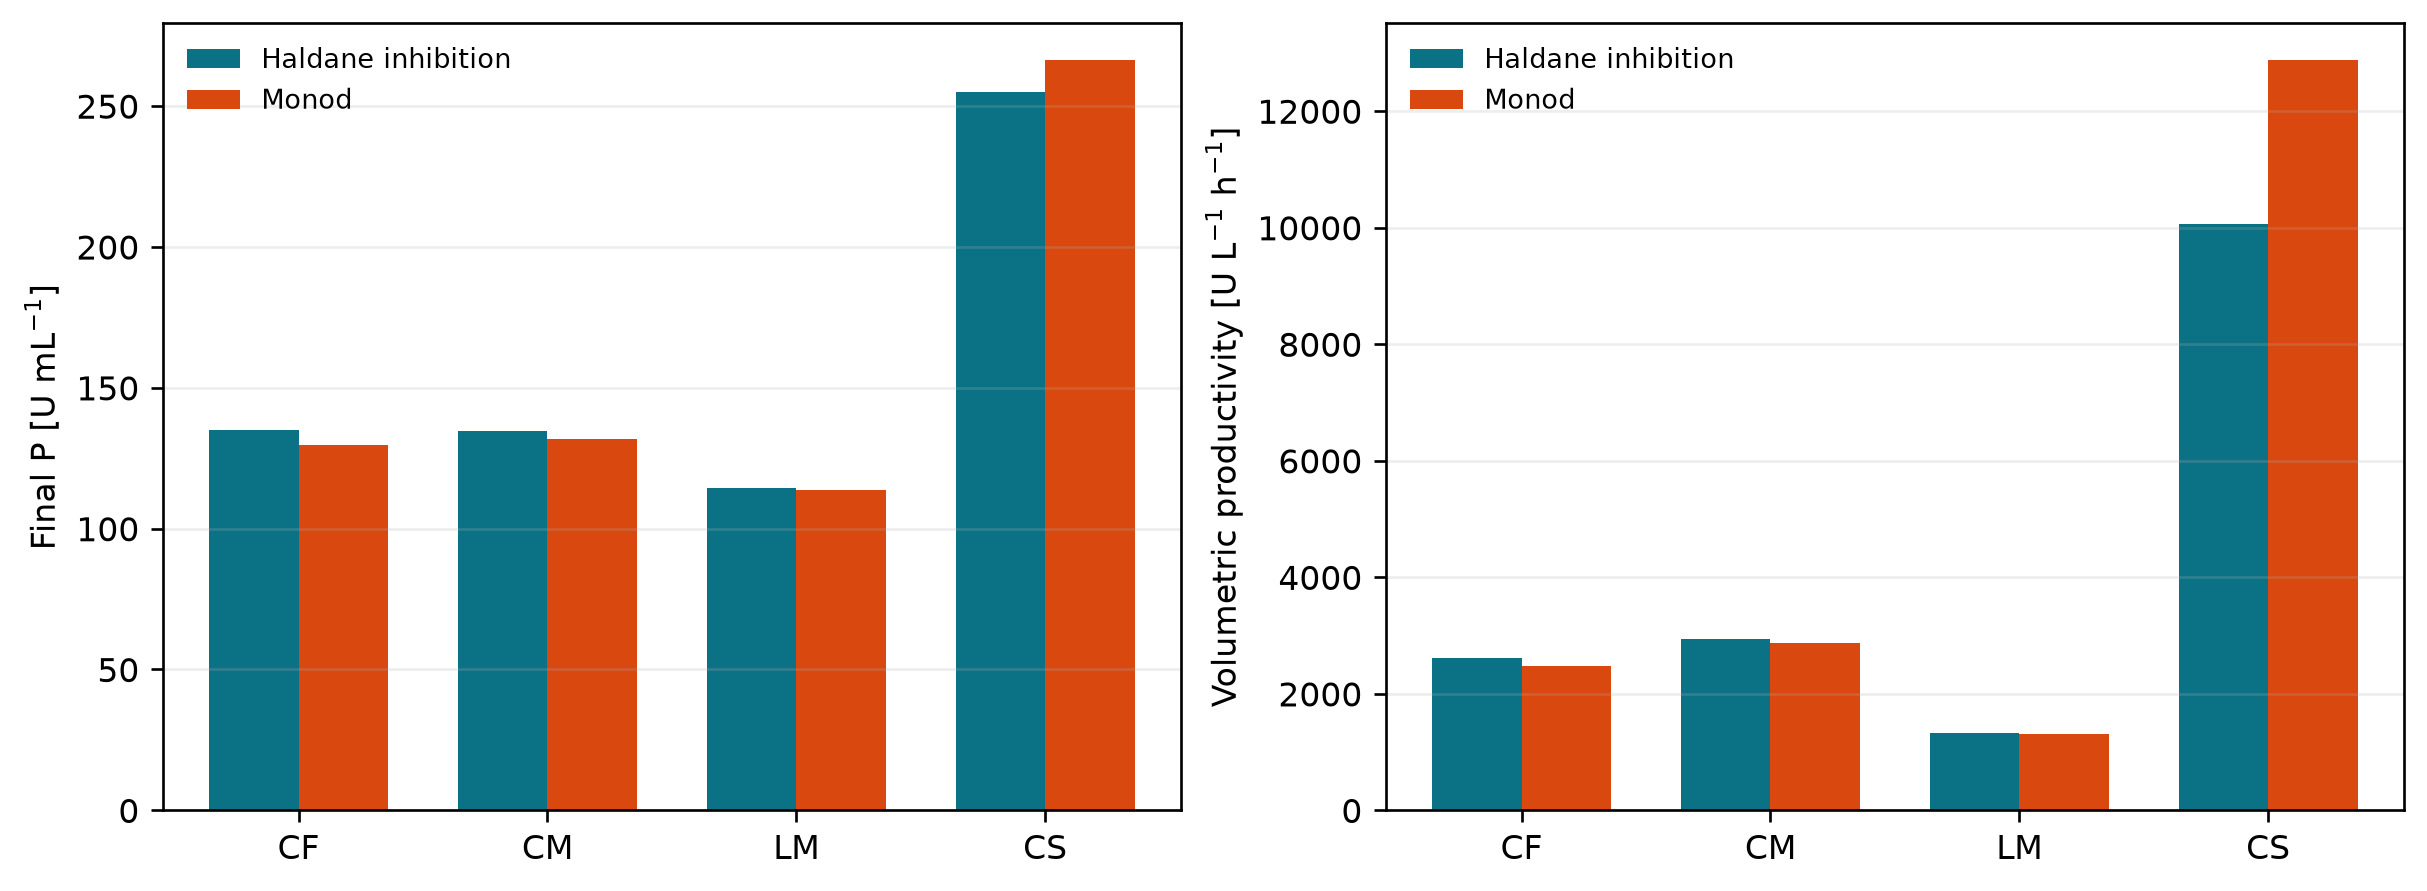
\includegraphics[width=0.90\textwidth]{figures/strategy_summary.png}
  \caption{Final product activity and volumetric productivity for all four strategies. The two model branches use identical process limits.}
  \label{fig:summary}
\end{figure}

\begin{figure}[t]
  \centering
  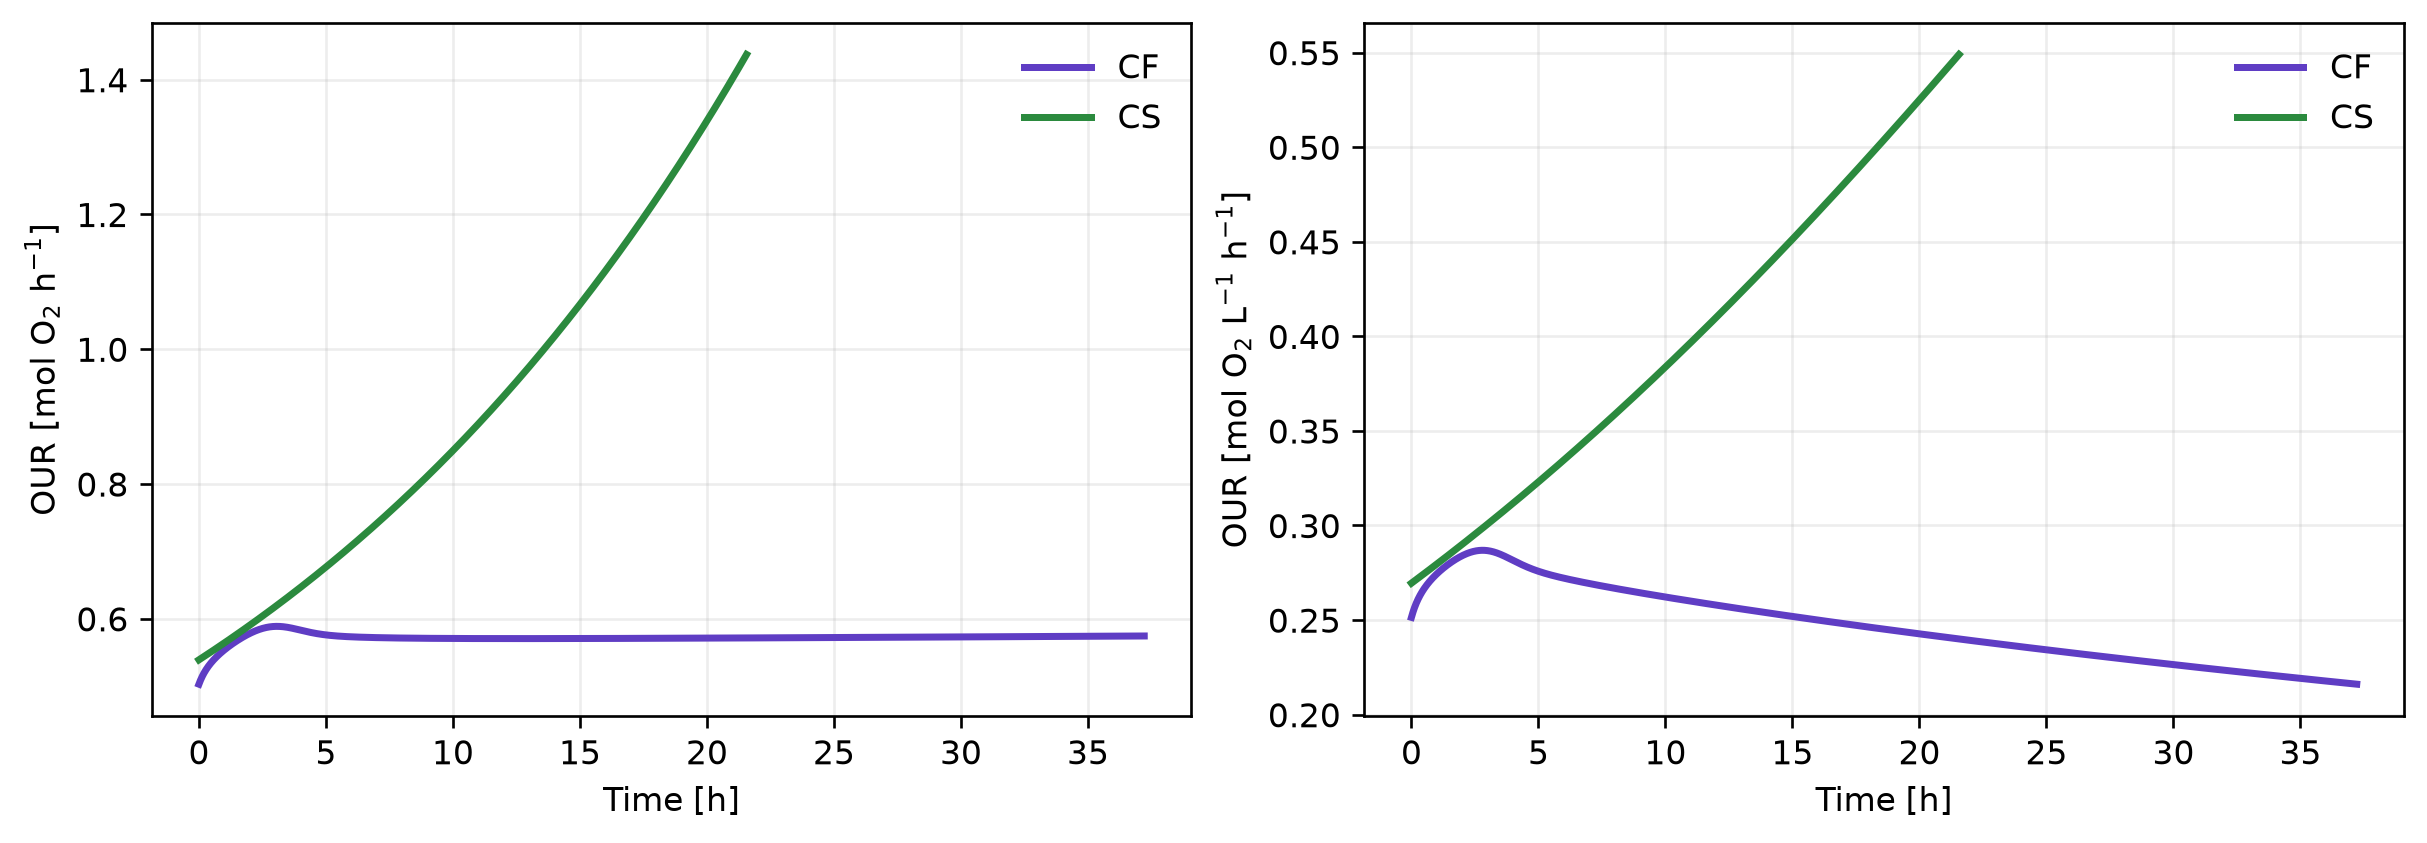
\includegraphics[width=0.88\textwidth]{figures/oxygen_demand.png}
  \caption{Derived oxygen demand for the inhibition branch. CS gives faster biomass and product formation, but it also creates the higher instantaneous oxygen requirement.}
  \label{fig:oxygen}
\end{figure}

\section{Conclusion and limitations}

This study presents a reproducible comparison of two substrate kinetic formulations in a four-state fed batch model. The parameter values and operating conditions were obtained from published work, while the dynamic simulations and performance calculations were carried out in the present implementation. The Monod formulation changes one modelling assumption while keeping the feed strategy, initial state, numerical solver, and process limits unchanged.

The results show why substrate inhibition matters in bioreactor operation. It changes the predicted productivity and prevents a high residual methanol concentration from being treated as universally beneficial. The derived oxygen calculation adds a practical reactor design consequence: the best product strategy also creates the largest oxygen demand and therefore needs an oxygen transfer check in the final project.

The main limitation is scope. The source model also discusses oxygen and carbon dioxide balances, gas transfer, and an adaptive predictive PI controller. The present analysis keeps oxygen as a derived demand and does not include a full OTR or $k_La$ design. It also does not reproduce the unpublished controller tuning parameters. These extensions can be added in a subsequent design stage.

\begin{thebibliography}{9}
\small
\setlength{\itemsep}{1pt}

\bibitem{Ponte2018}
X. Ponte, J. M. Barrigón, M. Maurer, D. Mattanovich, F. Valero, and J. L. Montesinos-Seguí, ``Towards optimal substrate feeding for heterologous protein production in \Ppastoris{} fed-batch processes under $P_{AOX1}$ control: a modeling aided approach,'' \textit{Journal of Chemical Technology and Biotechnology}, vol. 93, pp. 3208--3218, 2018. DOI: \href{https://doi.org/10.1002/jctb.5677}{10.1002/jctb.5677}.

\bibitem{PonteThesis}
X. Ponte, ``Towards optimal substrate feeding for heterologous protein production in \Ppastoris{} fed batch process under $P_{AOX1}$ control: a modelling aided approach,'' doctoral thesis, Universitat Autònoma de Barcelona, 2017. Accessible at \href{https://ddd.uab.cat/pub/tesis/2017/hdl_10803_457712/xpf1de1.pdf}{ddd.uab.cat/pub/tesis/2017/hdl\_10803\_457712/xpf1de1.pdf}.

\bibitem{IITBProject}
Indian Institute of Technology Bombay, ``CL 420 Upstream Bioprocess Project, Student Instructions,'' local course file, `moodle-content/CL420 Upstream Bioprocess Project - Student Instructions.pdf`.

\bibitem{IITBKickoff}
Indian Institute of Technology Bombay, ``CL 420 Biochemical Engineering Kickoff,'' local course file, `moodle-content/CL\_420\_Biochemical\_Engineering\_Kickoff.pdf`.

\bibitem{IITBModel}
Indian Institute of Technology Bombay, ``Structured Model V1,'' local course file, `moodle-content/Structured Model V1.pdf`.

\end{thebibliography}

\end{document}
